\section{Рабочий проект}

\subsection{Спецификация класса Course}

Модель Course хранит информацию о курсе, созданном преподавателем.

Описание: организует уроки и тесты, поддерживает мультиязычные названия и описания.

Валидация данных:
	\begin{itemize}
		\item поля title, description валидируются через CourseForm;
		\item поле image проверяется на формат (JPEG, PNG).
	\end{itemize}
	
Связи:
	\begin{itemize}
		\item внешний ключ creator на User;
		\item связан с Lesson, Enrollment.
	\end{itemize}
		
Безопасность:
	\begin{itemize}
		\item редактирование доступно только creator через CourseUpdateView;
		\item студенты видят только курсы с isactive=True.
	\end{itemize}
	
Уведомления:
	\begin{itemize}
		\item уведомления через Django messages (например, «Курс создан»).
	\end{itemize}
	
Основные методы:
	\begin{itemize}
		\item str(): возвращает title;
		\item getabsoluteurl(): возвращает URL курса;
		\item save(): обрабатывает изображение.
	\end{itemize}
	
Зависимости:
	\begin{itemize}
		\item связан с Lesson, Test, Enrollment;
		\item использует CKEditor для description.
	\end{itemize}

Описание полей класса Course приведено в табл. ~\ref {tab:course_attributes}

\begin{xltabular}{\textwidth}{|l|l|l|X|}
	\caption{Поля класса Course\label{tab:course_attributes}}\\
	\hline
	Поле & Тип & Обязательное & Описание \\ \hline
	\endfirsthead
	\continuecaption{Продолжение таблицы \ref{tab:course_attributes}}\\
	\hline
	Поле & Тип & Обязательное & Описание \\ \hline
	\endhead
	id & Integer & да & Уникальный идентификатор \\ \hline
	title & String & да & Название курса \\ \hline
	description & Text & нет & Описание (HTML, CKEditor) \\ \hline
	image & Image & нет & Изображение курса \\ \hline
	isactive & Boolean & да & Статус публикации \\ \hline
	creator & ForeignKey & да & Преподаватель (User) \\ \hline
\end{xltabular}

Описание методов класса Course приведено в табл. ~\ref {tab:course_methods}

\begin{xltabular}{\textwidth}{|l|X|}
	\caption{Методы класса Course\label{tab:course_methods}}\\
	\hline
	Метод & Описание \\ \hline
	\endfirsthead
	\continuecaption{Продолжение таблицы \ref{tab:course_methods}}\\
	\hline
	Метод & Описание \\ \hline
	\endhead
	str() & Возвращает title \\ \hline
	getabsoluteurl() & Возвращает URL курса \\ \hline
	save() & Обрабатывает изображение \\ \hline
\end{xltabular}

\begin{lstlisting}[language=Python, caption=Представление для создания курса, label=lst:course_view]
	from django.contrib.auth.decorators import login_required
	from django.shortcuts import render, redirect
	from .models import Course
	from .forms import CourseForm
	
	@login_required
	def create_course(request):
	if not request.user.is_teacher:
	return redirect('home')
	if request.method == 'POST':
	form = CourseForm(request.POST, request.FILES)
	if form.is_valid():
	course = form.save(commit=False)
	course.creator = request.user
	course.save()
	return redirect('courses')
	else:
	form = CourseForm()
	return render(request, 'courses/create.html', {'form': form})
\end{lstlisting}

\subsubsection{Спецификация класса Lesson}

Модель Lesson описывает урок в составе курса.

Описание: хранит контент, видео и упражнения, поддерживает мультиязычность.

Валидация данных:
	\begin{itemize}
		\item поля title, content валидируются через LessonForm;
		\item поле videourl проверяется на корректность.
	\end{itemize}
	
Связи:
	\begin{itemize}
		\item внешний ключ course на Course;
		\item связан с Test, StudentProgress.
	\end{itemize}
	
Безопасность:
	\begin{itemize}
		\item редактирование ограничено creator курса;
		\item доступ для студентов: ispublished=True.
	\end{itemize}
	
Уведомления:
	\begin{itemize}
		\item уведомления через Django messages (например, «Урок добавлен»).
	\end{itemize}
	
Основные методы:
	\begin{itemize}
		\item str(): возвращает title;
		\item save(): проверяет order.
	\end{itemize}
	
Зависимости:
	\begin{itemize}
		\item связан с Course, Test, StudentProgress;
		\item использует CKEditor для content.
	\end{itemize}

Описание полей класса Lesson приведено в табл. ~\ref {tab:lesson_attributes}

\begin{xltabular}{\textwidth}{|l|l|l|X|}
	\caption{Поля класса Lesson\label{tab:lesson_attributes}}\\
	\hline
	Поле & Тип & Обязательное & Описание \\ \hline
	\endfirsthead
	\continuecaption{Продолжение таблицы \ref{tab:lesson_attributes}}\\
	\hline
	Поле & Тип & Обязательное & Описание \\ \hline
	\endhead
	id & Integer & да & Уникальный идентификатор \\ \hline
	title & String & да & Название урока \\ \hline
	content & Text & да & Содержимое (HTML, CKEditor) \\ \hline
	videourl & URL & нет & Ссылка на видео \\ \hline
	order & Integer & да & Порядок урока \\ \hline
	ispublished & Boolean & да & Статус публикации \\ \hline
	exercise & Text & нет & Интерактивное упражнение \\ \hline
	expectedresult & Text & нет & Ожидаемый результат \\ \hline
	course & ForeignKey & да & Курс (Course) \\ \hline
\end{xltabular}

Описание методов класса Lesson приведено в табл. ~\ref {tab:lesson_methods}

\begin{xltabular}{\textwidth}{|l|X|}
	\caption{Методы класса Lesson\label{tab:lesson_methods}}\\
	\hline
	Метод & Описание \\ \hline
	\endfirsthead
	\continuecaption{Продолжение таблицы \ref{tab:lesson_methods}}\\
	\hline
	Метод & Описание \\ \hline
	\endhead
	str() & Возвращает title \\ \hline
	save() & Проверяет order \\ \hline
\end{xltabular}

\subsubsection{Спецификация класса Test}

Модель Test описывает тест, связанный с уроком.

Описание: проверяет знания студентов, поддерживает мультиязычные вопросы.

Валидация данных:
	\begin{itemize}
		\item поля title, description валидируются через TestForm;
		\item поле passingscore — положительное значение.
	\end{itemize}
	
Связи:
	\begin{itemize}
		\item внешний ключ lesson на Lesson;
		\item связан с Question, TestResult.
	\end{itemize}
	
Безопасность:
	\begin{itemize}
		\item редактирование ограничено creator урока;
		\item доступ для студентов: isactive=True.
	\end{itemize}
	
Уведомления:
	\begin{itemize}
		\item уведомления через Django messages (например, «Тест создан»).
	\end{itemize}
	
Основные методы:
	\begin{itemize}
		\item str(): возвращает title;
		\item save(): проверяет passingscore.
	\end{itemize}
	
Зависимости:
	\begin{itemize}
		\item связан с Lesson, Question, TestResult;
		\item используется в testform.html.
	\end{itemize}

Описание полей класса Test приведено в табл. ~\ref {tab:test_attributes}

\begin{xltabular}{\textwidth}{|l|l|l|X|}
	\caption{Поля класса Test\label{tab:test_attributes}}\\
	\hline
	Поле & Тип & Обязательное & Описание \\ \hline
	\endfirsthead
	\continuecaption{Продолжение таблицы \ref{tab:test_attributes}}\\
	\hline
	Поле & Тип & Обязательное & Описание \\ \hline
	\endhead
	id & Integer & да & Уникальный идентификатор \\ \hline
	title & String & да & Название теста \\ \hline
	description & Text & нет & Описание теста \\ \hline
	passingscore & Integer & да & Проходной балл \\ \hline
	isactive & Boolean & да & Статус активности \\ \hline
	lesson & ForeignKey & да & Урок (Lesson) \\ \hline
\end{xltabular}

Описание методов класса Test приведено в табл. ~\ref {tab:test_methods}

\begin{xltabular}{\textwidth}{|l|X|}
	\caption{Методы класса Test\label{tab:test_methods}}\\
	\hline
	Метод & Описание \\ \hline
	\endfirsthead
	\continuecaption{Продолжение таблицы \ref{tab:test_methods}}\\
	\hline
	Метод & Описание \\ \hline
	\endhead
	str() & Возвращает title \\ \hline
	save() & Проверяет passingscore \\ \hline
\end{xltabular}

\subsubsection{Спецификация класса Question}

Модель Question описывает вопрос в тесте.


Описание: поддерживает различные типы вопросов (одиночный, множественный, текстовый) с мультиязычным текстом.

Валидация данных:
	\begin{itemize}
		\item поле text валидируется через QuestionForm;
		\item поле questiontype принимает значения single, multiple, text;
		\item поле points проверяется на положительное значение.
	\end{itemize}
	
Связи:
	\begin{itemize}
		\item внешний ключ test на Test;
		\item связан с Answer.
	\end{itemize}
	
Безопасность:
	\begin{itemize}
		\item редактирование ограничено creator урока через представления;
		\item доступ для студентов только через активные тесты.
	\end{itemize}
	
Уведомления:
	\begin{itemize}
		\item уведомления через Django messages (например, «Вопрос добавлен»).
	\end{itemize}
	
Основные методы:
	\begin{itemize}
		\item str(): возвращает text;
		\item save(): проверяет questiontype и points.
	\end{itemize}
	
Зависимости:
	\begin{itemize}
		\item связан с Test, Answer;
		\item используется в шаблоне questionform.html.
	\end{itemize}

Описание полей класса Question приведено в табл. ~\ref {tab:question_attributes}

\begin{xltabular}{\textwidth}{|l|l|l|X|}
	\caption{Поля класса Question\label{tab:question_attributes}}\\
	\hline
	Поле & Тип & Обязательное & Описание \\ \hline
	\endfirsthead
	\continuecaption{Продолжение таблицы \ref{tab:question_attributes}}\\
	\hline
	Поле & Тип & Обязательное & Описание \\ \hline
	\endhead
	id & Integer & да & Уникальный идентификатор \\ \hline
	text & Text & да & Текст вопроса \\ \hline
	questiontype & String & да & Тип вопроса (single, multiple, text) \\ \hline
	points & Integer & да & Баллы за ответ \\ \hline
	test & ForeignKey & да & Тест (Test) \\ \hline
\end{xltabular}

Описание методов класса Question приведено в табл. ~\ref {tab:question_methods}

\begin{xltabular}{\textwidth}{|l|X|}
	\caption{Методы класса Question\label{tab:question_methods}}\\
	\hline
	Метод & Описание \\ \hline
	\endfirsthead
	\continuecaption{Продолжение таблицы \ref{tab:question_methods}}\\
	\hline
	Метод & Описание \\ \hline
	\endhead
	str() & Возвращает text \\ \hline
	save() & Проверяет questiontype и points \\ \hline
\end{xltabular}

\subsubsection{Спецификация класса Answer}

Модель Answer описывает вариант ответа на вопрос в тесте.

Описание: хранит текст ответа и флаг правильности, поддерживает мультиязычность.

Валидация данных:
	\begin{itemize}
		\item поле text валидируется через AnswerForm;
		\item поле iscorrect — булево, проверяется на уровне формы;
		\item поле order проверяется на положительное значение.
	\end{itemize}
	
Связи:
	\begin{itemize}
		\item внешний ключ question на Question;
		\item используется в TestResult.
	\end{itemize}
	
Безопасность:
	\begin{itemize}
		\item редактирование ограничено creator урока через AnswerCreateView;
		\item доступ для студентов только через активные тесты.
	\end{itemize}
	
Уведомления:
	\begin{itemize}
		\item уведомления через Django messages (например, «Ответ добавлен»).
	\end{itemize}
	
Лсновные методы:
	\begin{itemize}
		\item str(): возвращает text;
		\item save(): проверяет iscorrect и order.
	\end{itemize}
	
Зависимости:
	\begin{itemize}
		\item связан с Question, TestResult;
		\item используется в шаблоне answerform.html.
	\end{itemize}

Описание полей класса Answer приведено в табл. ~\ref {tab:answer_attributes}

\begin{xltabular}{\textwidth}{|l|l|l|X|}
	\caption{Поля класса Answer\label{tab:answer_attributes}}\\
	\hline
	Поле & Тип & Обязательное & Описание \\ \hline
	\endfirsthead
	\continuecaption{Продолжение таблицы \ref{tab:answer_attributes}}\\
	\hline
	Поле & Тип & Обязательное & Описание \\ \hline
	\endhead
	id & Integer & да & Уникальный идентификатор \\ \hline
	text & Text & да & Текст ответа \\ \hline
	iscorrect & Boolean & да & Признак правильности \\ \hline
	order & Integer & да & Порядок отображения \\ \hline
	question & ForeignKey & да & Вопрос (Question) \\ \hline
\end{xltabular}

Описание методов класса Answer приведено в табл. ~\ref {tab:answer_methods}

\begin{xltabular}{\textwidth}{|l|X|}
	\caption{Методы класса Answer\label{tab:answer_methods}}\\
	\hline
	Метод & Описание \\ \hline
	\endfirsthead
	\continuecaption{Продолжение таблицы \ref{tab:answer_methods}}\\
	\hline
	Метод & Описание \\ \hline
	\endhead
	str() & Возвращает text \\ \hline
	save() & Проверяет iscorrect и order \\ \hline
\end{xltabular}

\subsubsection{Спецификация класса TestResult}

Модель TestResult хранит результаты прохождения тестов студентами.


Описание: фиксирует баллы, выбранные ответы и дату завершения.

Валидация данных:
	\begin{itemize}
		\item поле score проверяется на положительное значение и соответствие максимуму теста;
		\item поле answers валидируется через TestSubmissionForm.
	\end{itemize}
	
Связи:
	\begin{itemize}
		\item внешний ключ student на User;
		\item внешний ключ lesson на Lesson;
		\item связь ManyToMany с Answer.
	\end{itemize}
	
Безопасность:
	\begin{itemize}
		\item доступ ограничен student или creator урока через представления;
		\item результаты видны только авторизованным пользователям.
	\end{itemize}
	
Уведомления:
	\begin{itemize}
		\item уведомления через Django messages (например, «Тест успешно пройден»).
	\end{itemize}
	
Основные методы:
	\begin{itemize}
		\item str(): возвращает информацию о результате (например, «Результат студента X по уроку Y»);
		\item save(): пересчитывает score на основе answers.
	\end{itemize}
	
Зависимости:
	\begin{itemize}
		\item связан с User, Lesson, Answer;
		\item используется в шаблоне testresult.html.
	\end{itemize}

Описание полей класса TestResult приведено в табл. ~\ref {tab:testresult_attributes}

\begin{xltabular}{\textwidth}{|l|l|l|X|}
	\caption{Поля класса TestResult\label{tab:testresult_attributes}}\\
	\hline
	Поле & Тип & Обязательное & Описание \\ \hline
	\endfirsthead
	\continuecaption{Продолжение таблицы \ref{tab:testresult_attributes}}\\
	\hline
	Поле & Тип & Обязательное & Описание \\ \hline
	\endhead
	id & Integer & да & Уникальный идентификатор \\ \hline
	student & ForeignKey & да & Студент (User) \\ \hline
	lesson & ForeignKey & да & Урок (Lesson) \\ \hline
	score & Integer & да & Полученные баллы \\ \hline
	answers & ManyToMany & да & Выбранные ответы \\ \hline
	attempts & Integer & да & Количество попыток \\ \hline
	completedat & DateTime & да & Дата завершения \\ \hline
\end{xltabular}

Описание методов класса TestResult приведено в табл. ~\ref {tab:testresult_methods}

\begin{xltabular}{\textwidth}{|l|X|}
	\caption{Методы класса TestResult\label{tab:testresult_methods}}\\
	\hline
	Метод & Описание \\ \hline
	\endfirsthead
	\continuecaption{Продолжение таблицы \ref{tab:testresult_methods}}\\
	\hline
	Метод & Описание \\ \hline
	\endhead
	str() & Возвращает информацию о результате \\ \hline
	save() & Пересчитывает score \\ \hline
\end{xltabular}

\subsubsection{Спецификация класса Enrollment}

Модель Enrollment фиксирует запись студента на курс.


Описание: связывает студента и курс для отслеживания участия.

Валидация данных:
	\begin{itemize}
		\item поля student и course проверяются на уникальность через uniquetogether.
	\end{itemize}
	
Связи:
	\begin{itemize}
		\item внешний ключ student на User;
		\item внешний ключ course на Course.
	\end{itemize}
	
Безопасность:
	\begin{itemize}
		\item доступ ограничен student или преподавателю через представления;
		\item преподаватели видят записи через teacherdashboard.
	\end{itemize}
	
Уведомления:
	\begin{itemize}
		\item уведомления через Django messages (например, «Вы записаны на курс»).
	\end{itemize}
	
Основные методы:
	\begin{itemize}
		\item str(): возвращает информацию о записи (например, «Студент X записан на курс Y»);
		\item save(): проверяет уникальность записи.
	\end{itemize}
	
Зависимости:
	\begin{itemize}
		\item связан с User, Course;
		\item используется в представлениях enrollcourse, unenrollcourse.
	\end{itemize}

Описание полей класса Enrollment приведено в табл. ~\ref {tab:enrollment_attributes}

\begin{xltabular}{\textwidth}{|l|l|l|X|}
	\caption{Поля класса Enrollment\label{tab:enrollment_attributes}}\\
	\hline
	Поле & Тип & Обязательное & Описание \\ \hline
	\endfirsthead
	\continuecaption{Продолжение таблицы \ref{tab:enrollment_attributes}}\\
	\hline
	Поле & Тип & Обязательное & Описание \\ \hline
	\endhead
	id & Integer & да & Уникальный идентификатор \\ \hline
	student & ForeignKey & да & Студент (User) \\ \hline
	course & ForeignKey & да & Курс (Course) \\ \hline
\end{xltabular}

Описание методов класса Enrollment приведено в табл. ~\ref {tab:enrollment_methods}

\begin{xltabular}{\textwidth}{|l|X|}
	\caption{Методы класса Enrollment\label{tab:enrollment_methods}}\\
	\hline
	Метод & Описание \\ \hline
	\endfirsthead
	\continuecaption{Продолжение таблицы \ref{tab:enrollment_methods}}\\
	\hline
	Метод & Описание \\ \hline
	\endhead
	str() & Возвращает информацию о записи \\ \hline
	save() & Проверяет уникальность \\ \hline
\end{xltabular}

\subsubsection{Спецификация класса StudentProgress}

Модель StudentProgress отслеживает прогресс студента по урокам.


Описание: фиксирует завершённость уроков и дату завершения.

Валидация данных:
	\begin{itemize}
		\item поле completed — булево, устанавливается через представления;
		\item поле completedat заполняется автоматически при completed=True.
	\end{itemize}
	
Связи:
	\begin{itemize}
		\item внешний ключ student на User;
		\item внешний ключ lesson на Lesson.
	\end{itemize}
	
Безопасность:
	\begin{itemize}
		\item доступ ограничен student через представления;
		\item преподаватели видят прогресс через teacherdashboard.
	\end{itemize}
	
Уведомления:
	\begin{itemize}
		\item уведомления через Django messages (например, «Урок завершён»).
	\end{itemize}
	
Основные методы:
	\begin{itemize}
		\item str(): возвращает информацию о прогрессе (например, «Прогресс студента X по уроку Y»);
		\item save(): устанавливает completedat.
	\end{itemize}
	
Зависимости:
	\begin{itemize}
		\item связан с User, Lesson;
		\item используется в представлениях completelesson, studentdashboard.
	\end{itemize}

Описание полей класса StudentProgress приведено в табл. ~\ref {tab:studentprogress_attributes}

\begin{xltabular}{\textwidth}{|l|l|l|X|}
	\caption{Поля класса StudentProgress\label{tab:studentprogress_attributes}}\\
	\hline
	Поле & Тип & Обязательное & Описание \\ \hline
	\endfirsthead
	\continuecaption{Продолжение таблицы \ref{tab:studentprogress_attributes}}\\
	\hline
	Поле & Тип & Обязательное & Описание \\ \hline
	\endhead
	id & Integer & да & Уникальный идентификатор \\ \hline
	student & ForeignKey & да & Студент (User) \\ \hline
	lesson & ForeignKey & да & Урок (Lesson) \\ \hline
	completed & Boolean & да & Завершённость урока \\ \hline
	completedat & DateTime & нет & Дата завершения \\ \hline
\end{xltabular}

Описание методов класса StudentProgress приведено в табл. ~\ref {tab:studentprogress_methods}

\begin{xltabular}{\textwidth}{|l|X|}
	\caption{Методы класса StudentProgress\label{tab:studentprogress_methods}}\\
	\hline
	Метод & Описание \\ \hline
	\endfirsthead
	\continuecaption{Продолжение таблицы \ref{tab:studentprogress_methods}}\\
	\hline
	Метод & Описание \\ \hline
	\endhead
	str() & Возвращает информацию о прогрессе \\ \hline
	save() & Устанавливает completedat \\ \hline
\end{xltabular}

\subsubsection{Спецификация класса Achievement}

Модель Achievement описывает достижения, присваиваемые студентам.


Описание: хранит информацию о наградах (например, «Первый завершённый урок»)).

Валидация данных:
	\begin{itemize}
		\item поля title, description валидируются через AchievementForm;
		\item проверка уникальности title через Django ORM.
	\end{itemize}
	
Связи:
	\begin{itemize}
		\item связан с UserAchievement через внешний ключ.
	\end{itemize}
	
Безопасность:
	\begin{itemize}
		\item редактирование ограничено администраторам через isstaff.
	\end{itemize}
	
Уведомления:
	\begin{itemize}
		\item уведомления через Django messages (например, «Достижение создано»).
	\end{itemize}
	
Основные методы:
	\begin{itemize}
		\item str(): возвращает title;
		\item save(): проверяет уникальность title.
	\end{itemize}
	
Зависимости:
	\begin{itemize}
		\item связан с UserAchievement;
		\item используется в studentdashboard.
	\end{itemize}

Описание полей класса Achievement приведено в табл. ~\ref {tab:achievement_attributes}

\begin{xltabular}{\textwidth}{|l|l|l|X|}
	\caption{Поля класса Achievement\label{tab:achievement_attributes}}\\
	\hline
	Поле & Тип & Обязательное & Описание \\ \hline
	\endfirsthead
	\continuecaption{Продолжение таблицы \ref{tab:achievement_attributes}}\\
	\hline
	Поле & Тип & Обязательное & Описание \\ \hline
	\endhead
	id & Integer & да & Уникальный идентификатор \\ \hline
	title & String & да & Название достижения \\ \hline
	description & Text & нет & Описание достижения \\ \hline
\end{xltabular}

Описание методов класса Achievement приведено в табл. ~\ref {tab:achievement_methods}

\begin{xltabular}{\textwidth}{|l|X|}
	\caption{Методы класса Achievement\label{tab:achievement_methods}}\\
	\hline
	Метод & Описание \\ \hline
	\endfirsthead
	\continuecaption{Продолжение таблицы \ref{tab:achievement_methods}}\\
	\hline
	Метод & Описание \\ \hline
	\endhead
	str() & Возвращает title \\ \hline
	save() & Проверяет уникальность title \\ \hline
\end{xltabular}

\subsubsection{Спецификация класса UserAchievement}

Модель UserAchievement связывает пользователей с достижениями.


Описание: отслеживает, какие достижения присвоены студентам.

Валидация данных:
	\begin{itemize}
		\item поля user и achievement проверяются на уникальность через uniquetogether.
	\end{itemize}
	
Связи:
	\begin{itemize}
		\item внешний ключ user на User;
		\item внешний ключ achievement на Achievement.
	\end{itemize}
	
Безопасность:
	\begin{itemize}
		\item доступ ограничен user через представления;
		\item преподаватели видят достижения через teacherdashboard.
	\end{itemize}
	
Уведомления:
	\begin{itemize}
		\item уведомления через Django messages (например, «Новое достижение получено»).
	\end{itemize}
	
Основные методы:
	\begin{itemize}
		\item str(): возвращает информацию о достижении (например, «Достижение X для пользователя Y»);
		\item save(): проверяет уникальность связи.
	\end{itemize}
	
Зависимости:
	\begin{itemize}
		\item связан с User, Achievement;
		\item используется в studentdashboard.
	\end{itemize}

Описание полей класса UserAchievement приведено в табл. ~\ref {tab:userachievement_attributes}

\begin{xltabular}{\textwidth}{|l|l|l|X|}
	\caption{Поля класса UserAchievement\label{tab:userachievement_attributes}}\\
	\hline
	Поле & Тип & Обязательное & Описание \\ \hline
	\endfirsthead
	\continuecaption{Продолжение таблицы \ref{tab:userachievement_attributes}}\\
	\hline
	Поле & Тип & Обязательное & Описание \\ \hline
	\endhead
	id & Integer & да & Уникальный идентификатор \\ \hline
	user & ForeignKey & да & Пользователь (User) \\ \hline
	achievement & ForeignKey & да & Достижение (Achievement) \\ \hline
	awardedat & DateTime & да & Дата присвоения \\ \hline
\end{xltabular}

Описание методов класса UserAchievement приведено в табл. ~\ref {tab:userachievement_methods}

\begin{xltabular}{\textwidth}{|l|X|}
	\caption{Методы класса UserAchievement\label{tab:userachievement_methods}}\\
	\hline
	Метод & Описание \\ \hline
	\endfirsthead
	\continuecaption{Продолжение таблицы \ref{tab:userachievement_methods}}\\
	\hline
	Метод & Описание \\ \hline
	\endhead
	str() & Возвращает информацию о достижении \\ \hline
	save() & Проверяет уникальность связи \\ \hline
\end{xltabular}

\subsection{Модульное тестирование классов и методов программы}

Модульное тестирование проводилось для проверки корректности работы всех классов и методов обучающей платформы, разработанной на Django. Тестирование выполнялось с использованием фреймворка django.test, который позволяет создавать изолированные тестовые сценарии для моделей, представлений и форм.

Тестируемые компоненты:
\begin{enumerate}
	\item Модуль User: проверка создания пользователей с ролями студента и преподавателя.
	\begin{lstlisting}[language=Python, caption=Модульный тест для User, label=lst:user_test]
		from django.test import TestCase
		from django.contrib.auth import get_user_model
		
		User = get_user_model()
		
		class UserTestCases(TestCase):
		def setUp(self):
		self.teacher = User.objects.create_user(
		username='sonya1',
		password='vanya232323',
		is_teacher=True
		)
		self.student = User.objects.create_user(
		username='Ivan_Sedih',
		password='vanya232323',
		is_student=True
		)
		
		def test_user_creation(self):
		self.assertTrue(self.teacher.is_teacher)
		self.assertTrue(self.student.is_student)
	\end{lstlisting}
	
	\item Модуль Course: проверка создания курса, валидации полей и связи с создателем.
	\begin{lstlisting}[language=Python, caption=Модульный тест для Course, label=lst:course_test]
		from django.test import TestCase
		from learning.models import Course
		from django.contrib.auth import get_user_model
		
		User = get_user_model()
		
		class CourseTestCases(TestCase):
		def setUp(self):
		self.teacher = User.objects.create_user(username='sonya1', password='vanya232323', is_teacher=True)
		self.course = Course.objects.create(
		title='Основы JS',
		description='Описание курса',
		creator=self.teacher,
		is_active=True
		)
		
		def test_course_creation(self):
		self.assertEqual(self.course.title, 'Основы JS')
		self.assertEqual(self.course.creator, self.teacher)
		self.assertTrue(self.course.is_active)
	\end{lstlisting}
	
	\item Модуль Lesson: проверка добавления урока, порядка и связи с курсом.
	\begin{lstlisting}[language=Python, caption=Модульный тест для Lesson, label=lst:lesson_test]
		from django.test import TestCase
		from learning.models import Course, Lesson
		from django.contrib.auth import get_user_model
		
		User = get_user_model()
		
		class LessonTestCases(TestCase):
		def setUp(self):
		self.teacher = User.objects.create_user(username='sonya1', password='vanya232323', is_teacher=True)
		self.course = Course.objects.create(title='Массивы', description='Описание курса', creator=self.teacher)
		self.lesson = Lesson.objects.create(
		title='Что такое массивы',
		content='Содержимое урока',
		order=1,
		course=self.course,
		is_published=True
		)
		
		def test_lesson_creation(self):
		self.assertEqual(self.lesson.title, 'Что такое массивы')
		self.assertEqual(self.lesson.order, 1)
		self.assertEqual(self.lesson.course, self.course)
	\end{lstlisting}
	
	\item Модуль Test: проверка создания тестов и связи с уроком.
	\begin{lstlisting}[language=Python, caption=Модульный тест для Test, label=lst:test_test]
		from django.test import TestCase
		from learning.models import Test, Lesson, Course
		from django.contrib.auth import get_user_model
		
		User = get_user_model()
		
		class TestTestCases(TestCase):
		def setUp(self):
		self.teacher = User.objects.create_user(username='sonya1', password='vanya232323', is_teacher=True)
		self.course = Course.objects.create(title='Массивы', description='Описание курса', creator=self.teacher)
		self.lesson = Lesson.objects.create(title='Поиск индекса элемента в массиве', content='Содержимое урока', order=1, course=self.course)
		self.test = Test.objects.create(
		title='Тест',
		passing_score=80,
		lesson=self.lesson,
		is_active=True
		)
		
		def test_test_creation(self):
		self.assertEqual(self.test.title, 'Тест')
		self.assertEqual(self.test.passing_score, 80)
		self.assertEqual(self.test.lesson, self.lesson)
	\end{lstlisting}
	
	\item Модуль TestResult: проверка сохранения результатов тестов.
	\begin{lstlisting}[language=Python, caption=Модульный тест для TestResult, label=lst:testresult_test]
		from django.test import TestCase
		from learning.models import TestResult, Test, Lesson, Course
		from django.contrib.auth import get_user_model
		from django.utils import timezone
		
		User = get_user_model()
		
		class TestResultTestCases(TestCase):
		def setUp(self):
		self.teacher = User.objects.create_user(username='sonya1', password='vanya232323', is_teacher=True)
		self.student = User.objects.create_user(username='Ivan_Sedih', password='vanya232323', is_student=True)
		self.course = Course.objects.create(title='Объекты', description='Описание курса', creator=self.teacher)
		self.lesson = Lesson.objects.create(title='Создание объектов', content='Содержимое урока', order=1, course=self.course)
		self.test = Test.objects.create(title='Тест', passing_score=70, lesson=self.lesson)
		self.test_result = TestResult.objects.create(
		student=self.student,
		lesson=self.lesson,
		score=85,
		answers='{"q1": "a1"}',
		attempts=1,
		completed_at=timezone.now()
		)
		
		def test_testresult_creation(self):
		self.assertEqual(self.test_result.score, 85)
		self.assertEqual(self.test_result.student, self.student)
		self.assertEqual(self.test_result.lesson, self.lesson)
	\end{lstlisting}
	
	\item Модуль StudentProgress: проверка отметки о завершении урока.
	\begin{lstlisting}[language=Python, caption=Модульный тест для StudentProgress, label=lst:studentprogress_test]
		from django.test import TestCase
		from learning.models import StudentProgress, Lesson, Course
		from django.contrib.auth import get_user_model
		from django.utils import timezone
		
		User = get_user_model()
		
		class StudentProgressTestCases(TestCase):
		def setUp(self):
		self.teacher = User.objects.create_user(username='sonya1', password='vanya232323', is_teacher=True)
		self.student = User.objects.create_user(username='Ivan_Sedih', password='vanya232323', is_student=True)
		self.course = Course.objects.create(title='Типы данных', description='Описание курса', creator=self.teacher)
		self.lesson = Lesson.objects.create(title='Переменные', content='Содержимое урока', order=1, course=self.course)
		self.progress = StudentProgress.objects.create(
		student=self.student,
		lesson=self.lesson,
		completed=True,
		completed_at=timezone.now()
		)
		
		def test_studentprogress_creation(self):
		self.assertTrue(self.progress.completed)
		self.assertEqual(self.progress.student, self.student)
		self.assertEqual(self.progress.lesson, self.lesson)
	\end{lstlisting}
	
	\item Модуль UserAchievement: проверка присвоения достижений пользователям.
	\begin{lstlisting}[language=Python, caption=Модульный тест для UserAchievement, label=lst:userachievement_test]
		from django.test import TestCase
		from learning.models import Achievement, UserAchievement
		from django.contrib.auth import get_user_model
		from django.utils import timezone
		
		User = get_user_model()
		
		class UserAchievementTestCases(TestCase):
		def setUp(self):
		self.student = User.objects.create_user(username='Ivan_Sedih', password='vanya232323', is_student=True)
		self.achievement = Achievement.objects.create(
		title='Завершение теста',
		description='Сдан первый тест',
		badge_image='badges/test_completed.png'
		)
		self.user_achievement = UserAchievement.objects.create(
		user=self.student,
		achievement=self.achievement,
		awarded_at=timezone.now()
		)
		
		def test_userachievement_creation(self):
		self.assertEqual(self.user_achievement.user, self.student)
		self.assertEqual(self.user_achievement.achievement, self.achievement)
	\end{lstlisting}
\end{enumerate}

Инструменты: django.test.TestCase, unittest.\\
Результаты: все тесты выполнены успешно, ошибок не обнаружено.


\subsection{Системное тестирование разработанного веб-приложения}

Системное тестирование проводилось для проверки взаимодействия компонентов и интерфейса.

Сценарии тестирования:
	\begin{enumerate}
	\item Регистрация и авторизация пользователя.
	\item Создание курса и запись студента.
	\item Добавление урока с контентом через CKEditor.
	\item Прохождение теста и просмотр результатов.
	\item Присвоение достижения студенту.
	\item Редактирование курса.
	\item Удаление курса.
	\item Переупорядочивание уроков.
	\item Проверка доступа к уроку.
	\item Просмотр прогресса студента.
	\item Управление вопросами и ответами теста.
	\end{enumerate}


Описание сценариев тестирования:


	
\subsubsection{Регистрация и авторизация пользователя}
	
Описание: пользователь должен иметь возможность зарегистрироваться в системе, выбрав роль (преподаватель или студент), и войти с использованием учетных данных (имя пользователя, пароль, email).
	
Ожидаемый результат: при успешной регистрации и вводе верных учетных данных осуществляется вход, открывается главная рабочая область (панель управления для преподавателя или каталог курсов для студента). При вводе некорректных данных система отображает сообщение об ошибке (например, "Пользователь не найден").
	
	\begin{figure}[ht]
		\centering
		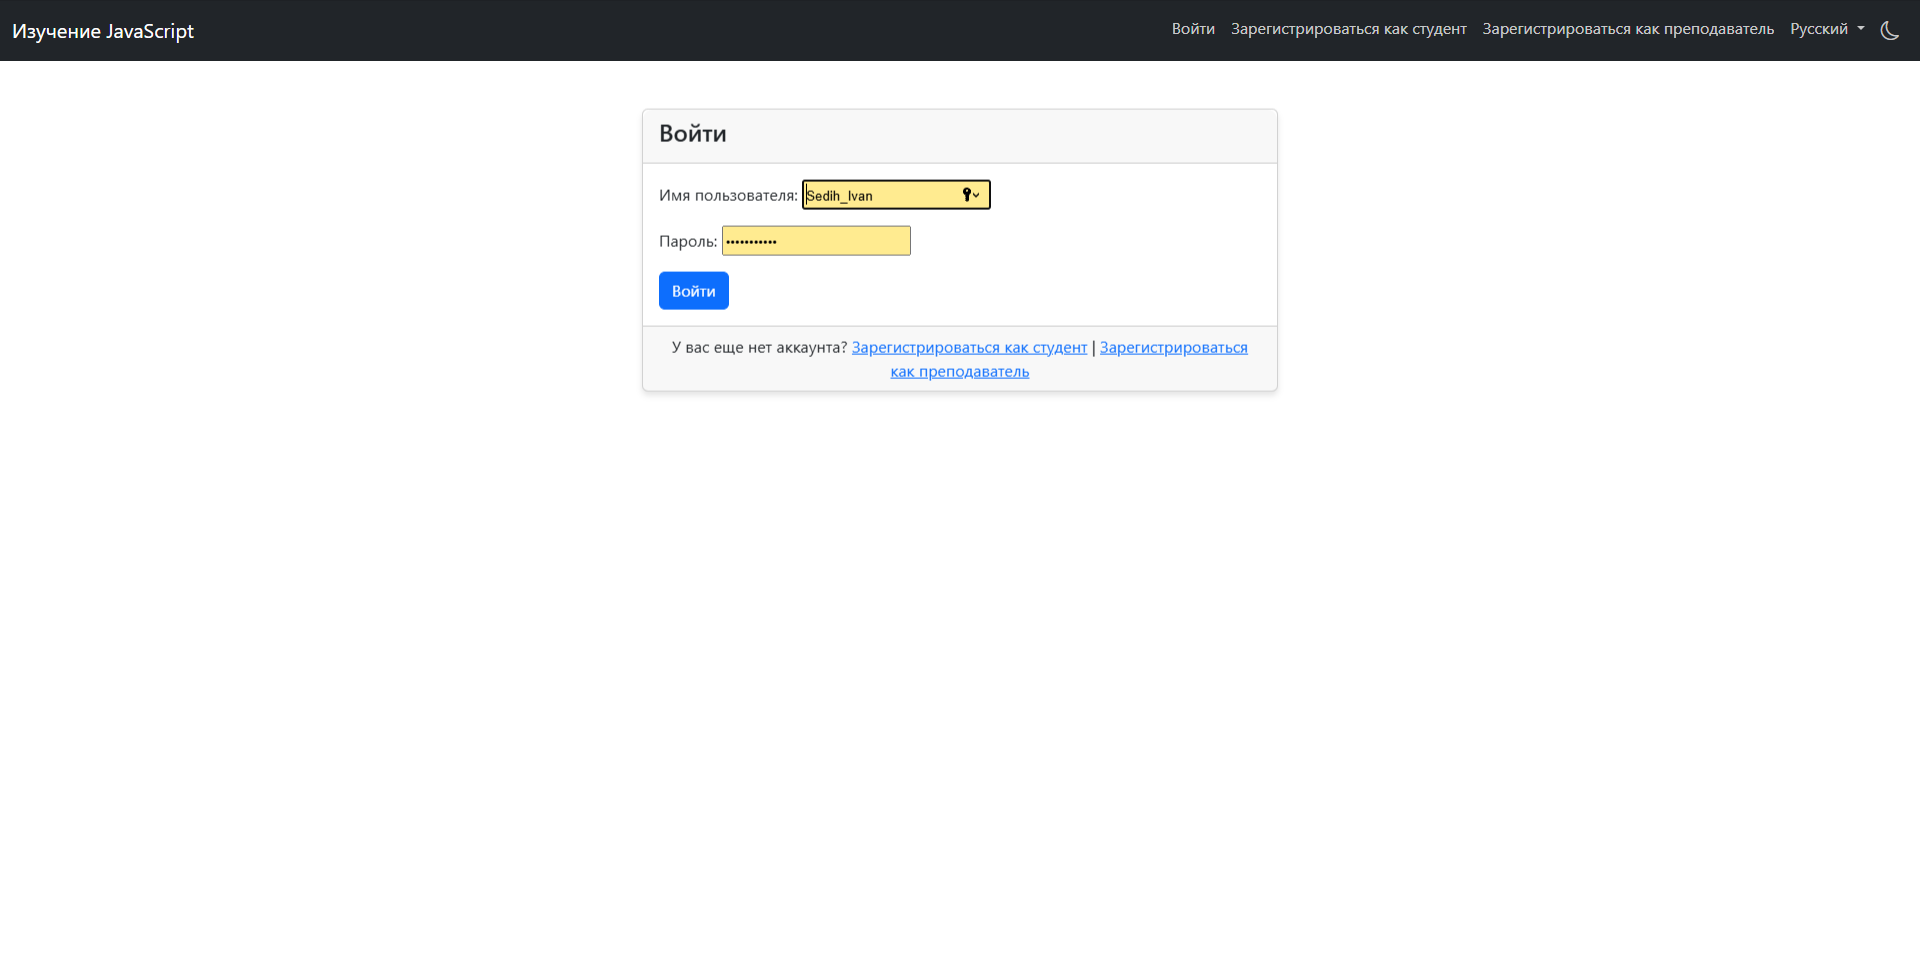
\includegraphics[width=0.9\textwidth]{images/регистр} 
		\caption{Регистрация и авторизация пользователя}
		\label{login:image}
	\end{figure}
	
\subsubsection{Создание курса и запись студента}
	
Описание: преподаватель должен иметь возможность создать новый курс, указав название, описание и изображение, а студент — записаться на существующий курс.
	
Ожидаемый результат: после создания курса он отображается в каталоге курсов, а студент, выбрав курс и нажав "Записаться", получает доступ к нему. При ошибке в данных (например, пустое название) система выдает предупреждение.
	
\begin{figure}[ht]
		\centering
		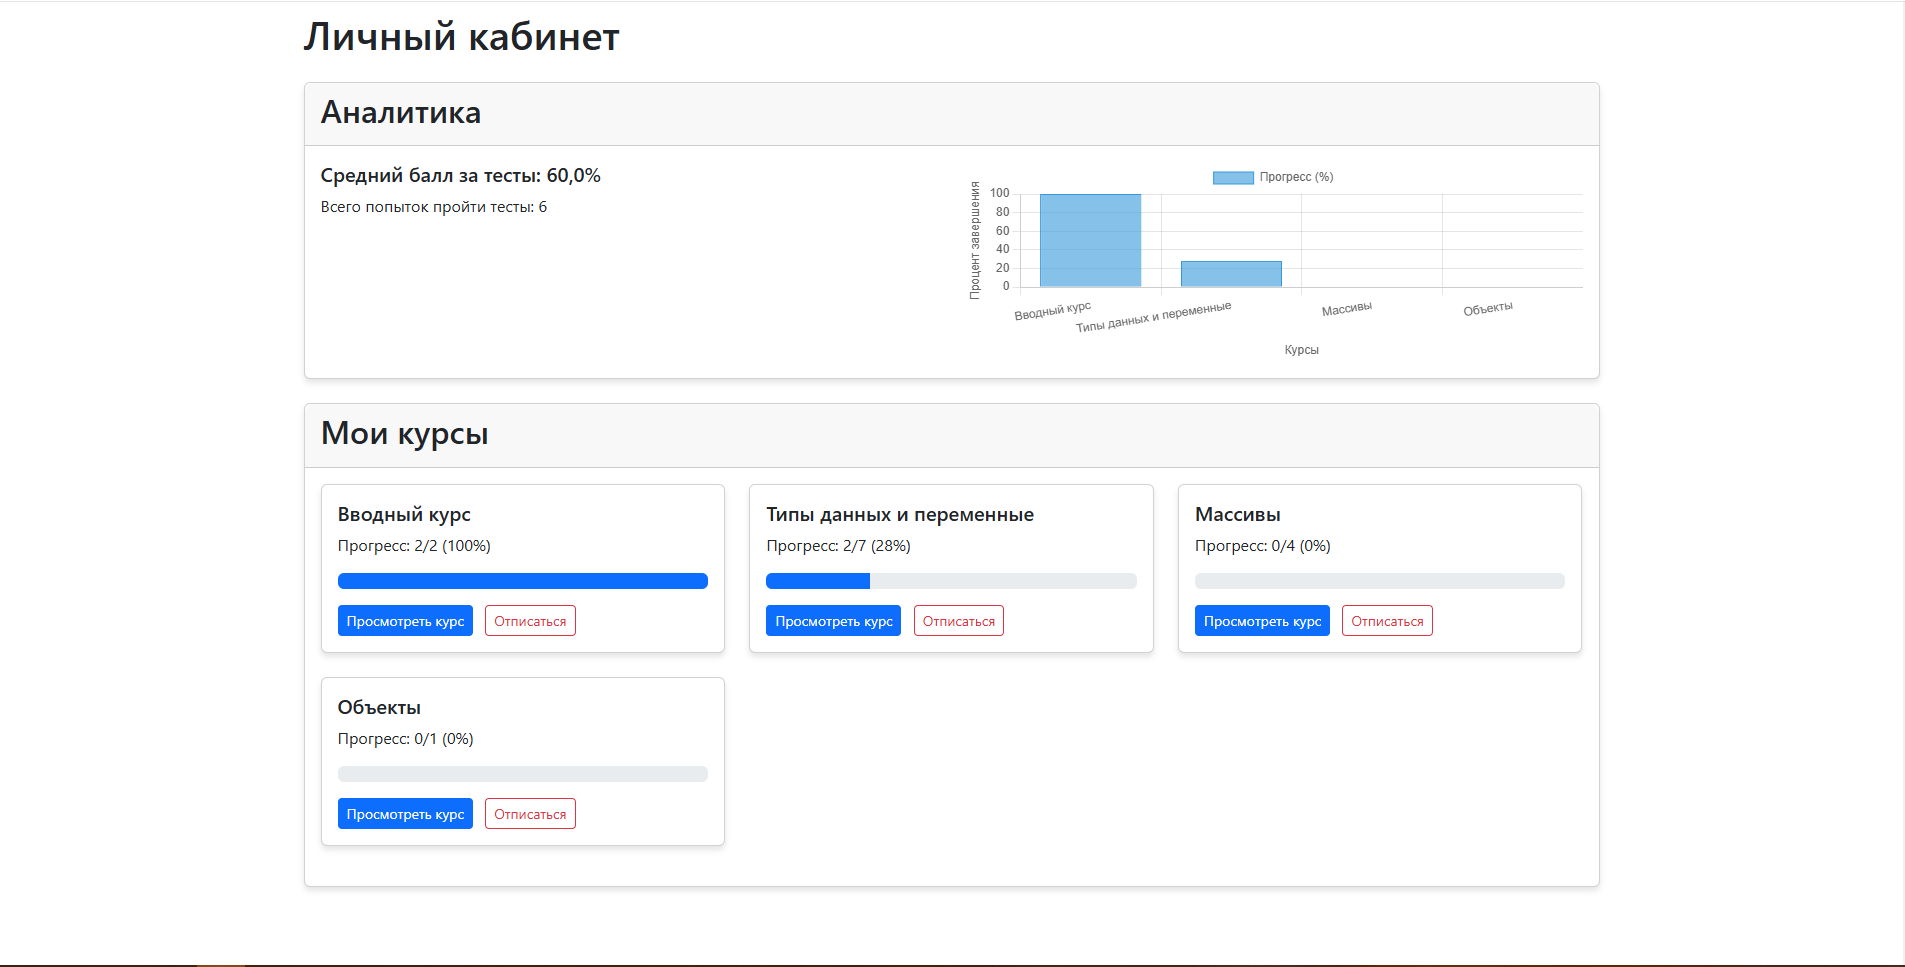
\includegraphics[width=0.9\textwidth]{images/запись} 
		\caption{Создание курса и запись студента}
		\label{enroll:image}
\end{figure}
	
\subsubsection{Добавление урока}
	
Описание: преподаватель должен иметь возможность добавить урок к курсу, используя CKEditor для редактирования контента (текст, видео, упражнения), с указанием порядка и статуса публикации.
	
Ожидаемый результат: урок успешно добавляется, контент отображается корректно для студентов после публикации. При отсутствии обязательных полей (например, названия) система выдает сообщение об ошибке.
	
	\begin{figure}[ht]
		\centering
		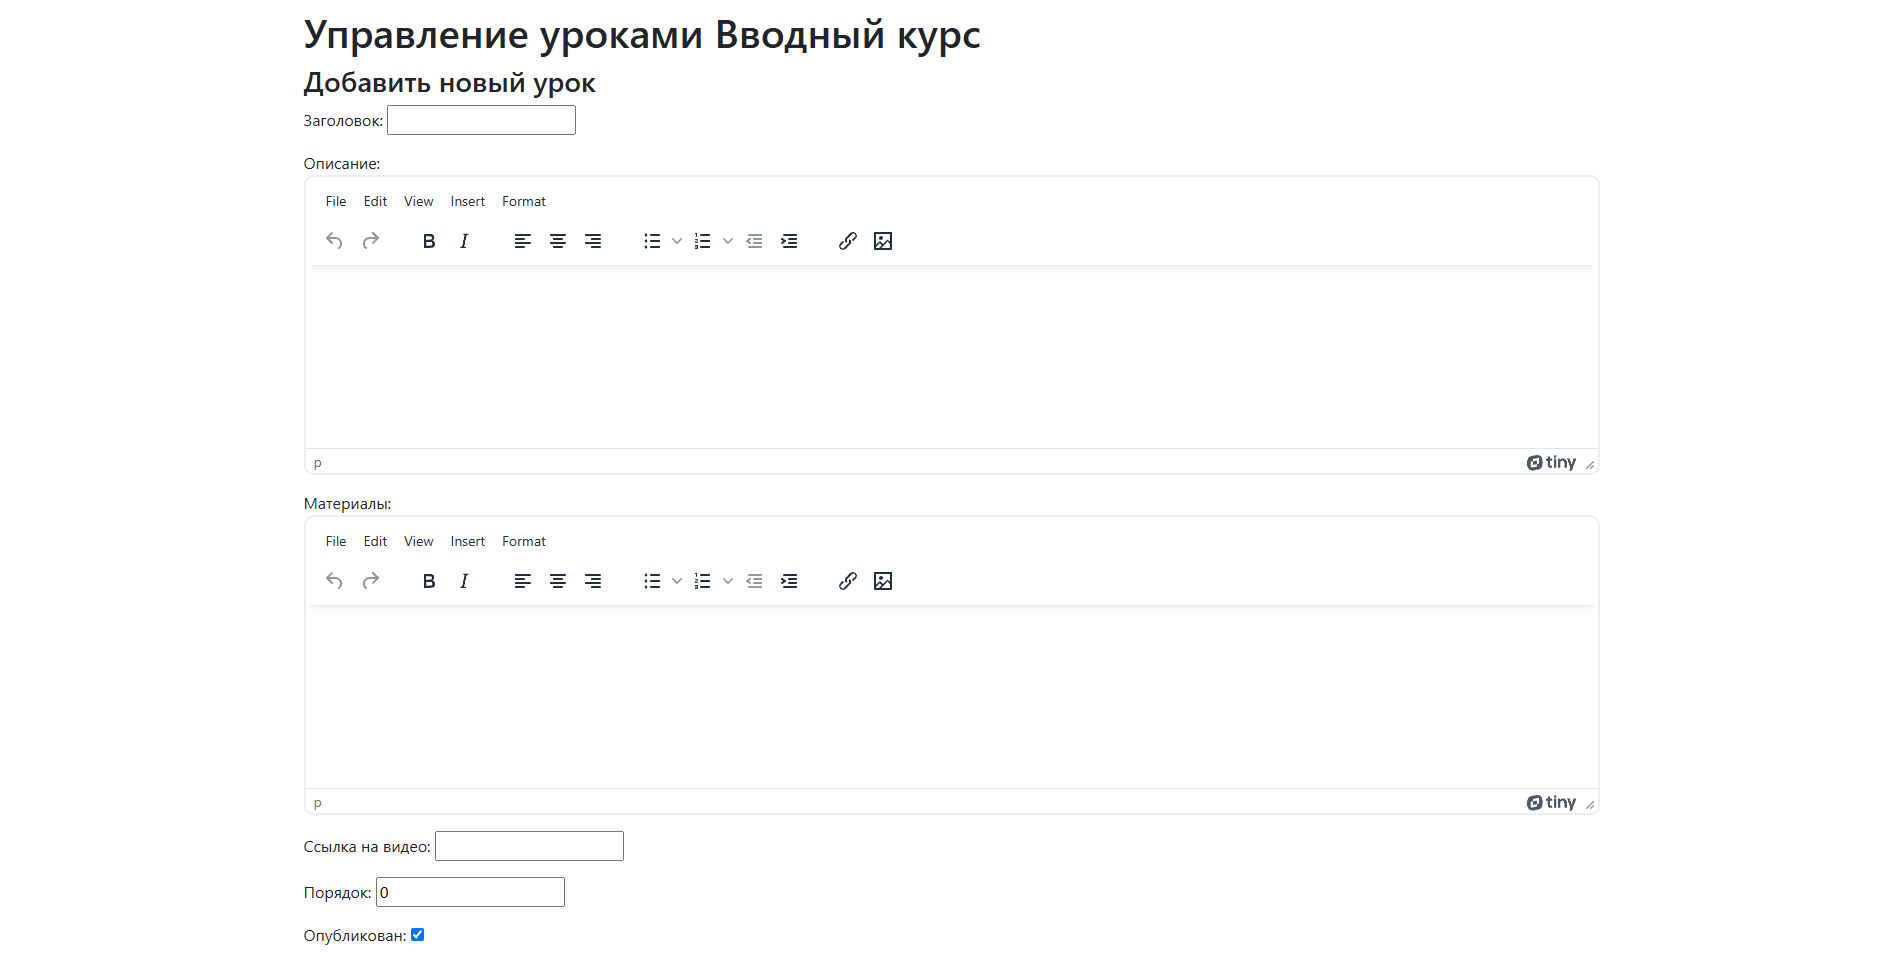
\includegraphics[width=0.9\textwidth]{images/урокдобавить} 
		\caption{Добавление урока}
		\label{urok:image}
	\end{figure}
\newpage
\subsubsection{Прохождение теста и просмотр результатов}
	
Описание: студент должен иметь возможность пройти тест, связанный с уроком, выбрав ответы или введя текст, и просмотреть результат после завершения.
	
Ожидаемый результат: после сдачи теста отображаются баллы и статус (пройден/не пройден). При некорректных ответах система сохраняет результат и предлагает повторить попытку, если разрешено.
	
	\begin{figure}[ht]
		\centering
		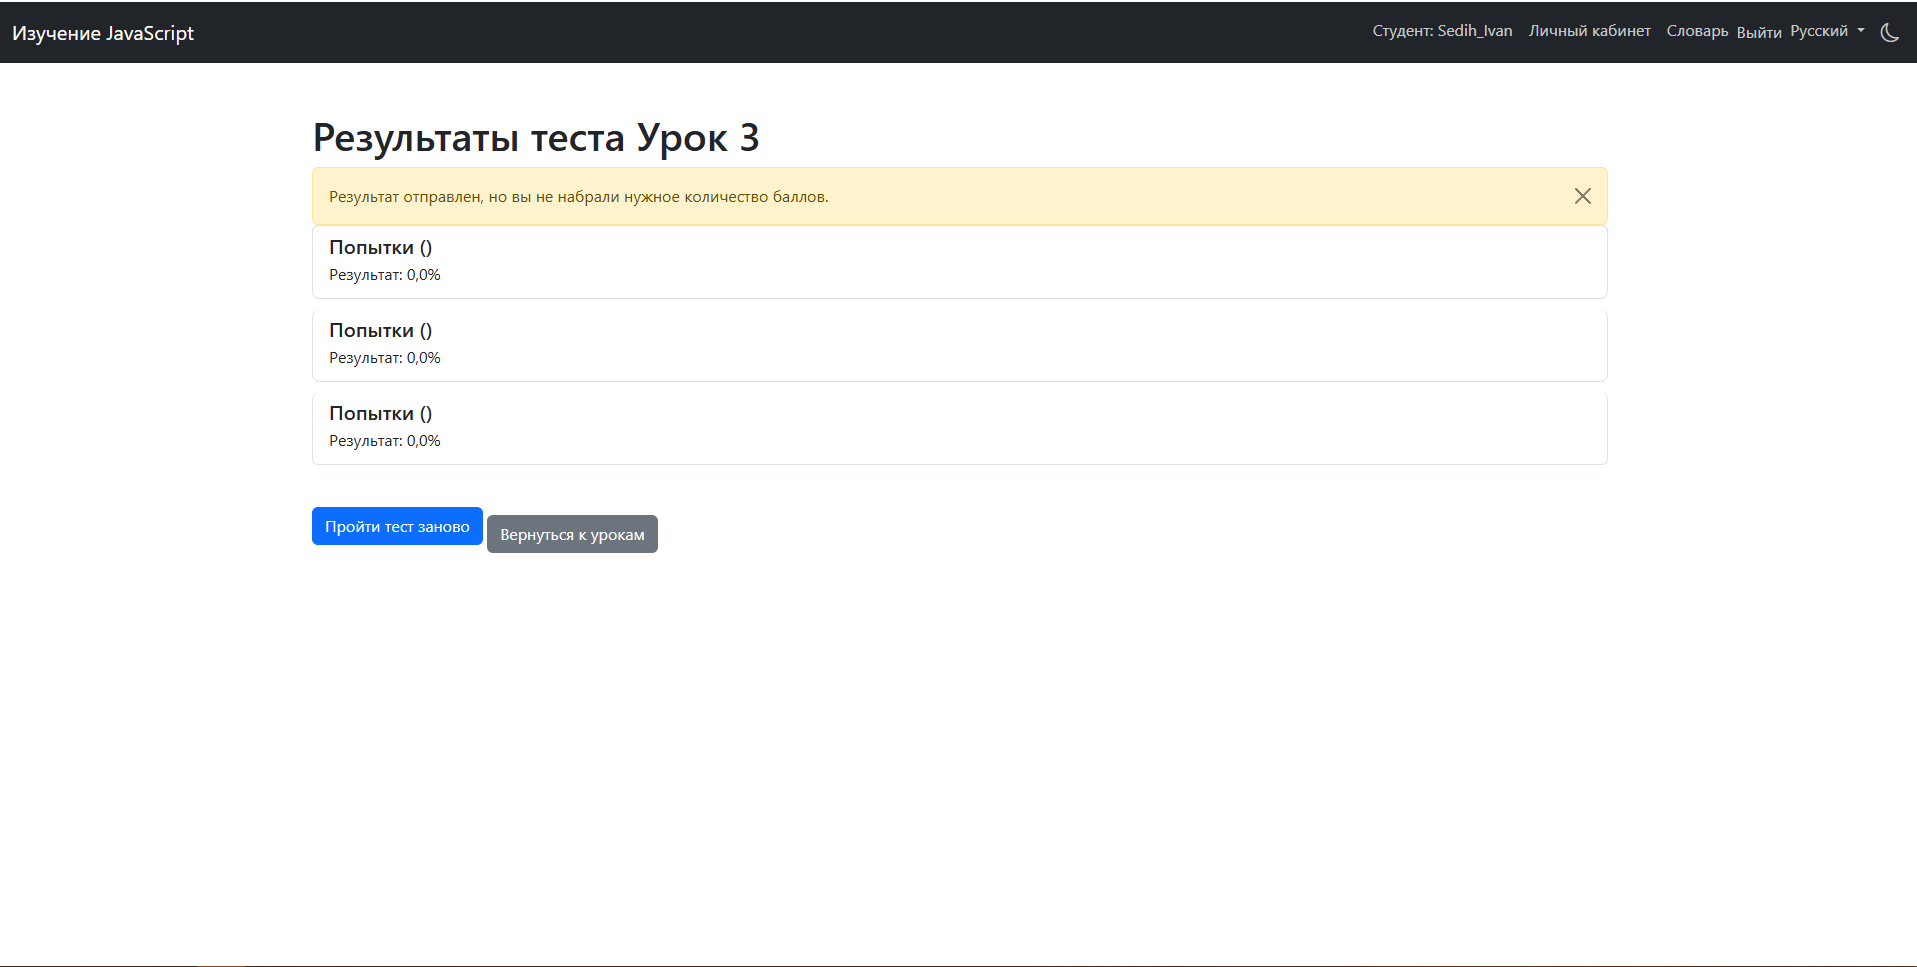
\includegraphics[width=0.9\textwidth]{images/тестрез} 
		\caption{Прохождение теста и результаты}
		\label{test:image}
	\end{figure}
	
\subsubsection{Присвоение достижения студенту}
	
Описание: система должна автоматически присваивать достижение студенту после выполнения определенного действия (например, завершения первого урока), а студент должен иметь возможность просмотреть полученные достижения в своем профиле.
	
Ожидаемый результат: после завершения урока система регистрирует достижение (например, "Первый завершённый урок") и отображается его в профиле студента. При ошибке (например, если достижение не настроено) система уведомляет администратора, но не прерывает работу.
	
	\begin{figure}[ht]
		\centering
		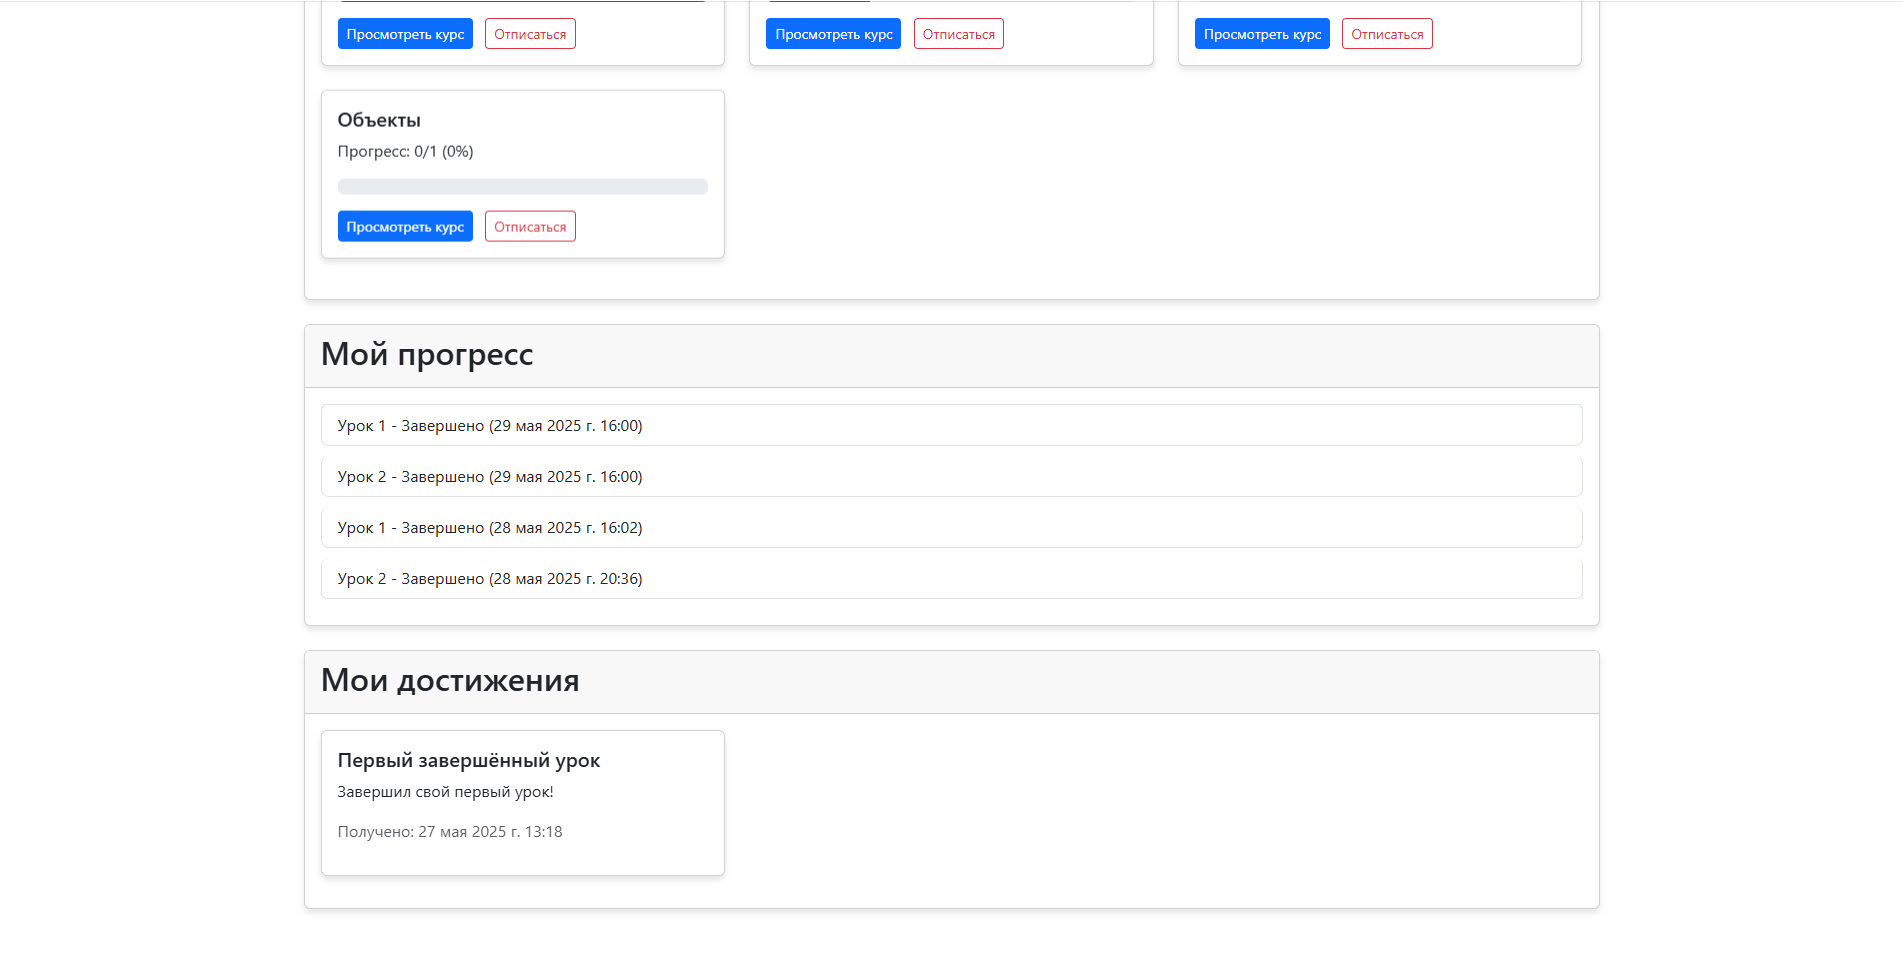
\includegraphics[width=0.9\textwidth]{images/достижение} 
		\caption{Присвоение достижения студенту}
		\label{achiv:image}
	\end{figure}
	
\subsubsection{Редактирование курса}
	
Описание: преподаватель должен иметь возможность редактировать существующий курс, изменяя его название, описание, изображение или статус публикации.
	
Ожидаемый результат: после редактирования изменения сохраняются, и обновленный курс отображается в каталоге курсов. При ошибке (например, пустое название) система выдает предупреждение.
	
	\begin{figure}[ht]
		\centering
		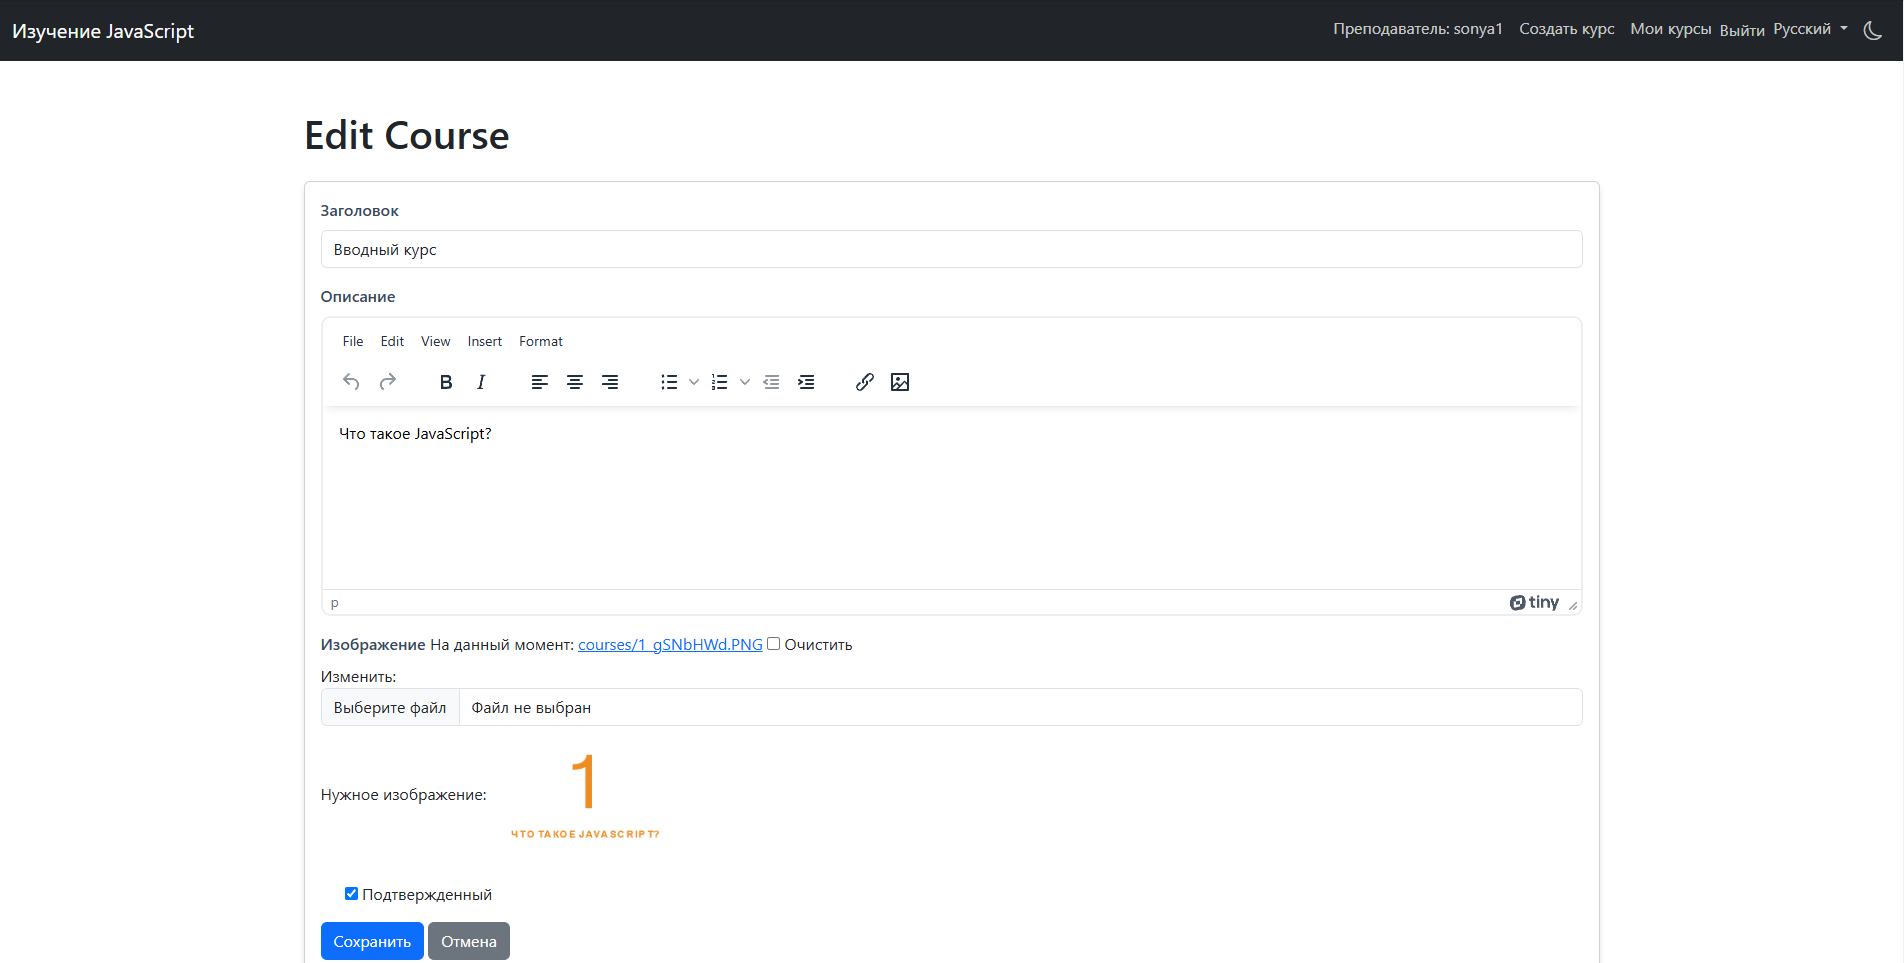
\includegraphics[width=0.9\textwidth]{images/редактироватькурс} 
		\caption{Редактирование курса}
		\label{editcourse:image}
	\end{figure}
	
\subsubsection{Удаление курса}
	
Описание: преподаватель должен иметь возможность удалить курс, при этом связанные данные (уроки, тесты) удаляются каскадно.
	
Ожидаемый результат: курс удаляется из системы, он больше не отображается в каталоге курсов, связанные уроки и тесты также удалены. При отсутствии прав (например, пользователь не является создателем курса) система выдает сообщение об ошибке.
	
	\begin{figure}[ht]
		\centering
		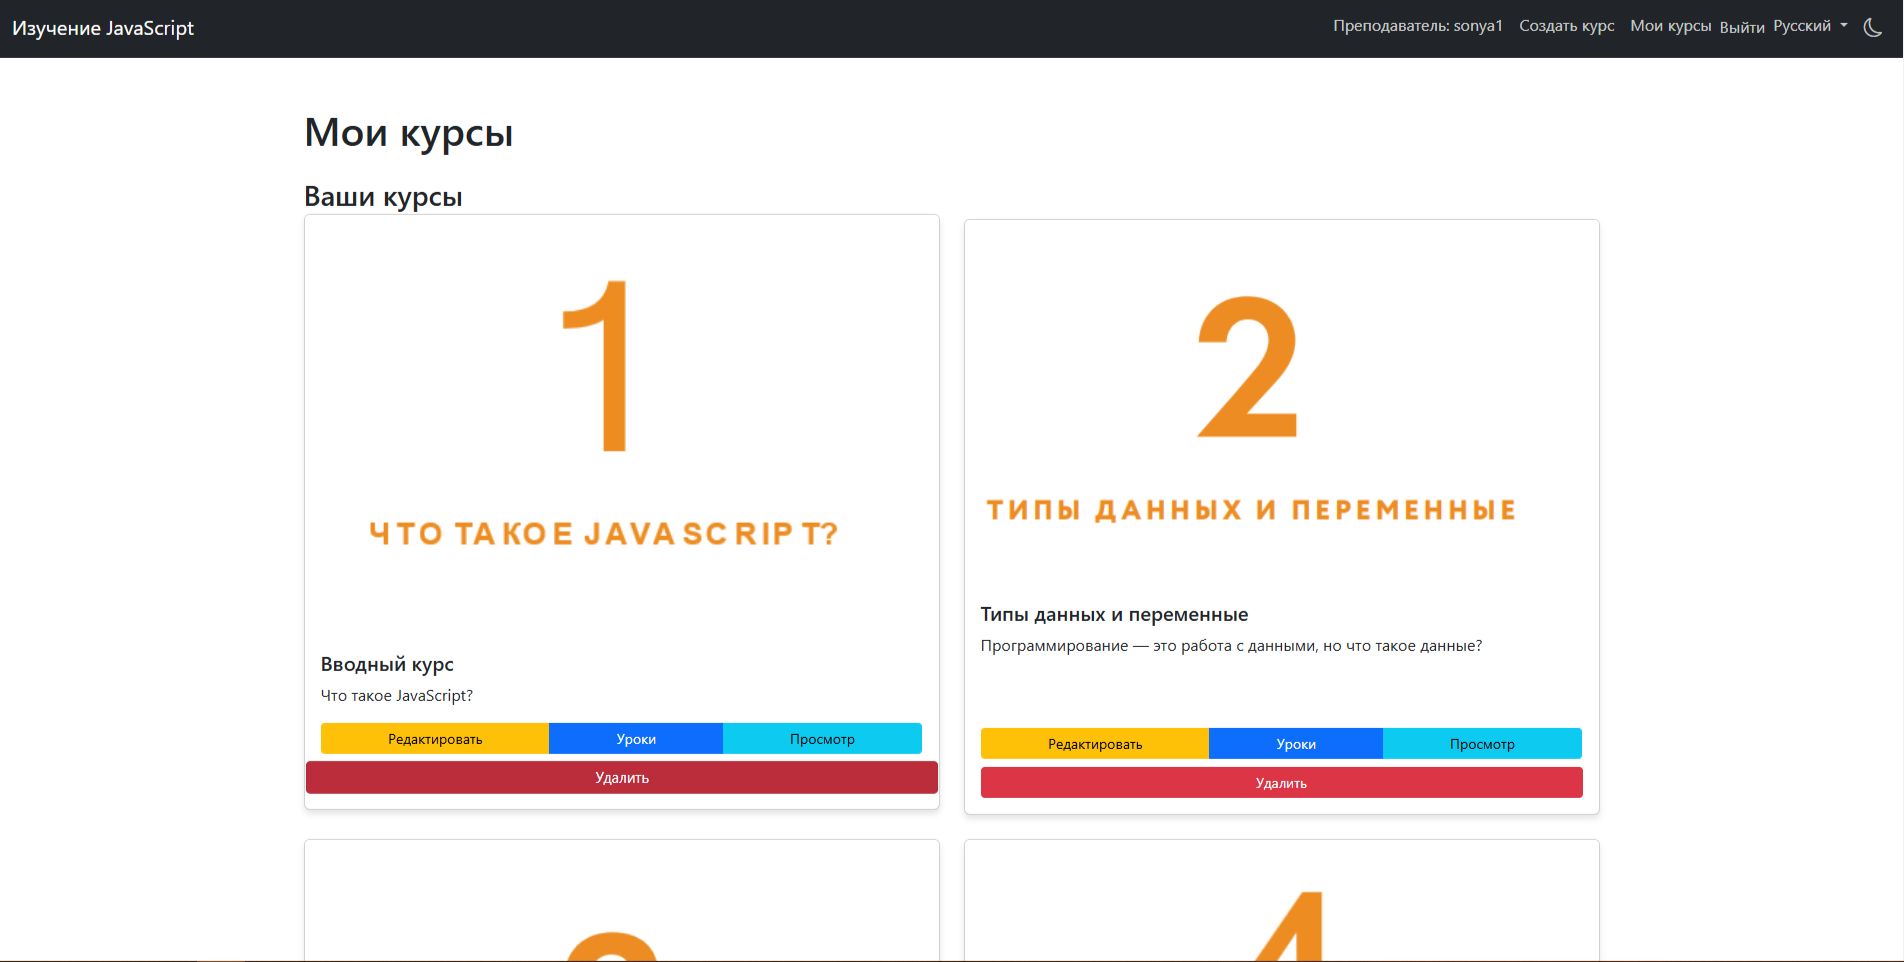
\includegraphics[width=0.9\textwidth]{images/удалитькурс} 
		\caption{Удаление курса}
		\label{deletecourse:image}
	\end{figure}
	
\subsubsection{Проверка доступа к уроку}
	
Описание: система должна ограничивать доступ студента к уроку, если предыдущий урок не завершен или тест не сдан.
	
Ожидаемый результат: студент не может открыть урок, если не выполнены условия доступа, и получает уведомление (например, "Завершите предыдущий урок"). При выполнении условий урок становится доступным.
	
	\begin{figure}[ht]
		\centering
		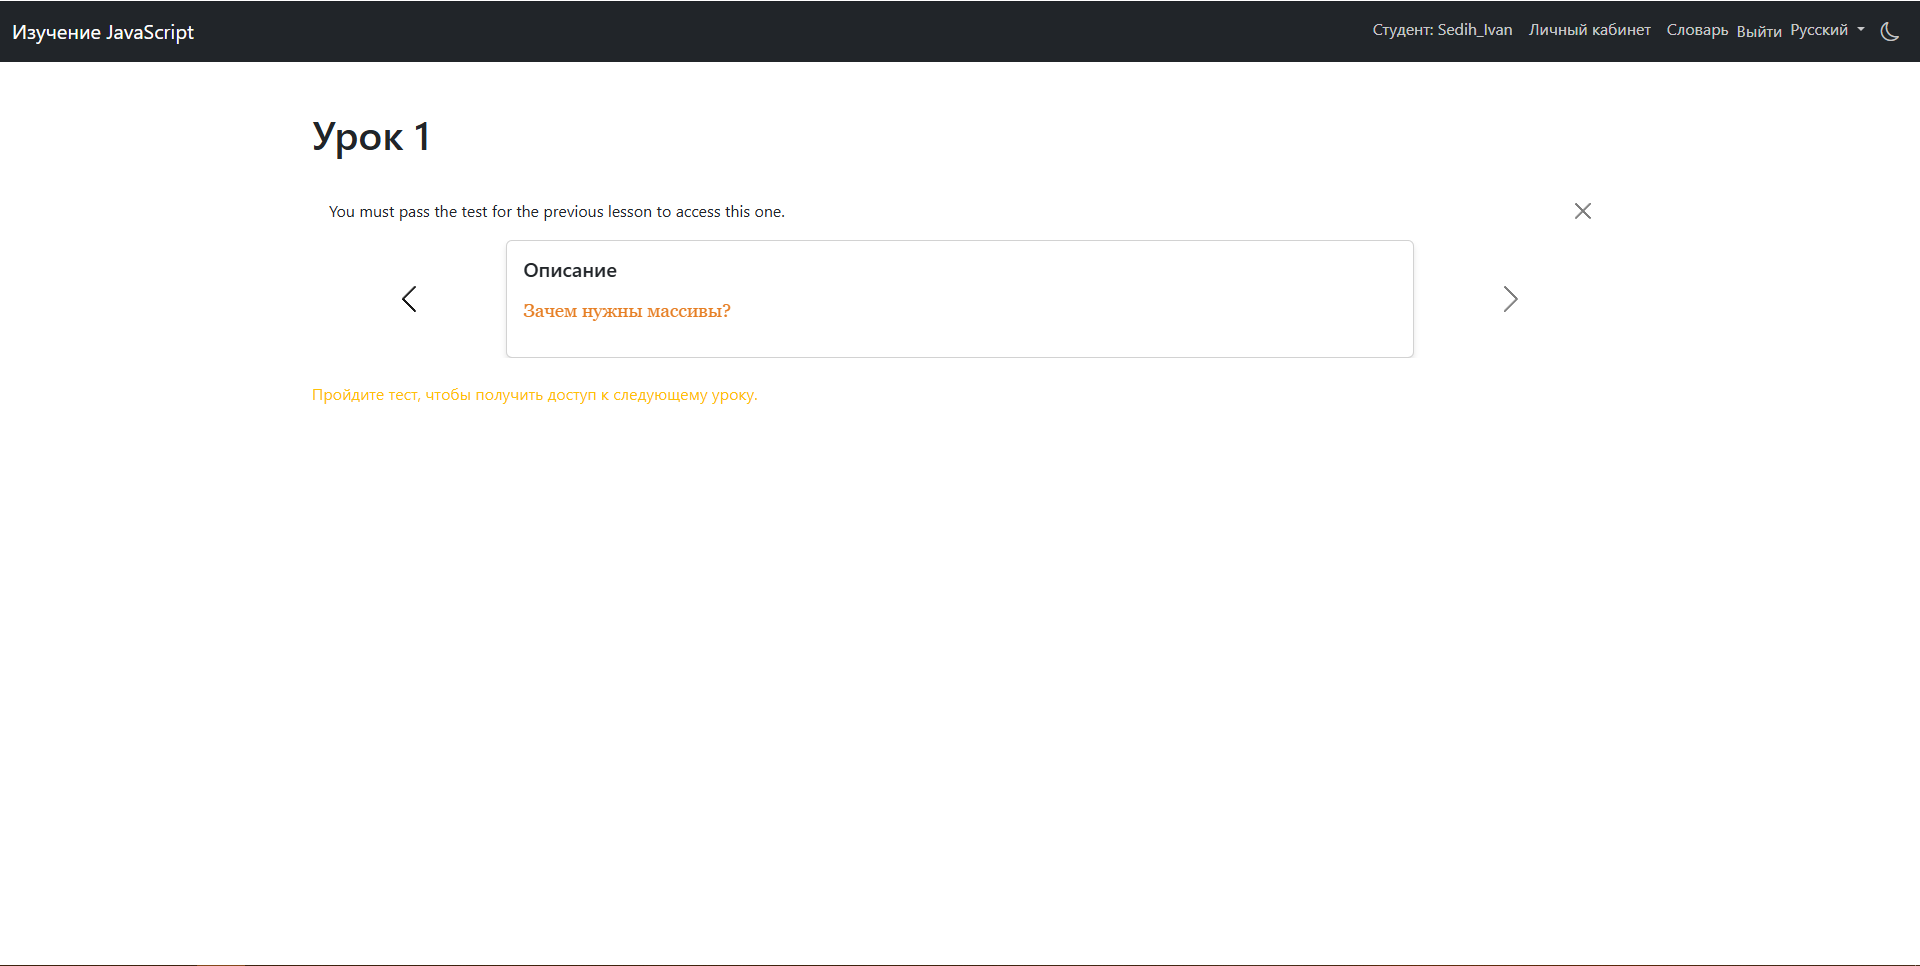
\includegraphics[width=0.9\textwidth]{images/доступурок} 
		\caption{Проверка доступа к уроку}
		\label{access:image}
	\end{figure}
	
\subsubsection{Просмотр прогресса студента}
	
Описание: студент должен иметь возможность просмотреть свой прогресс по курсу, включая завершенные уроки, результаты тестов и средний балл.
	
Ожидаемый результат: в панели студента отображаются завершенные уроки, результаты тестов и средний балл по курсу. При отсутствии данных (например, студент не начал курс) отображается соответствующее сообщение.
	
	\begin{figure}[ht]
		\centering
		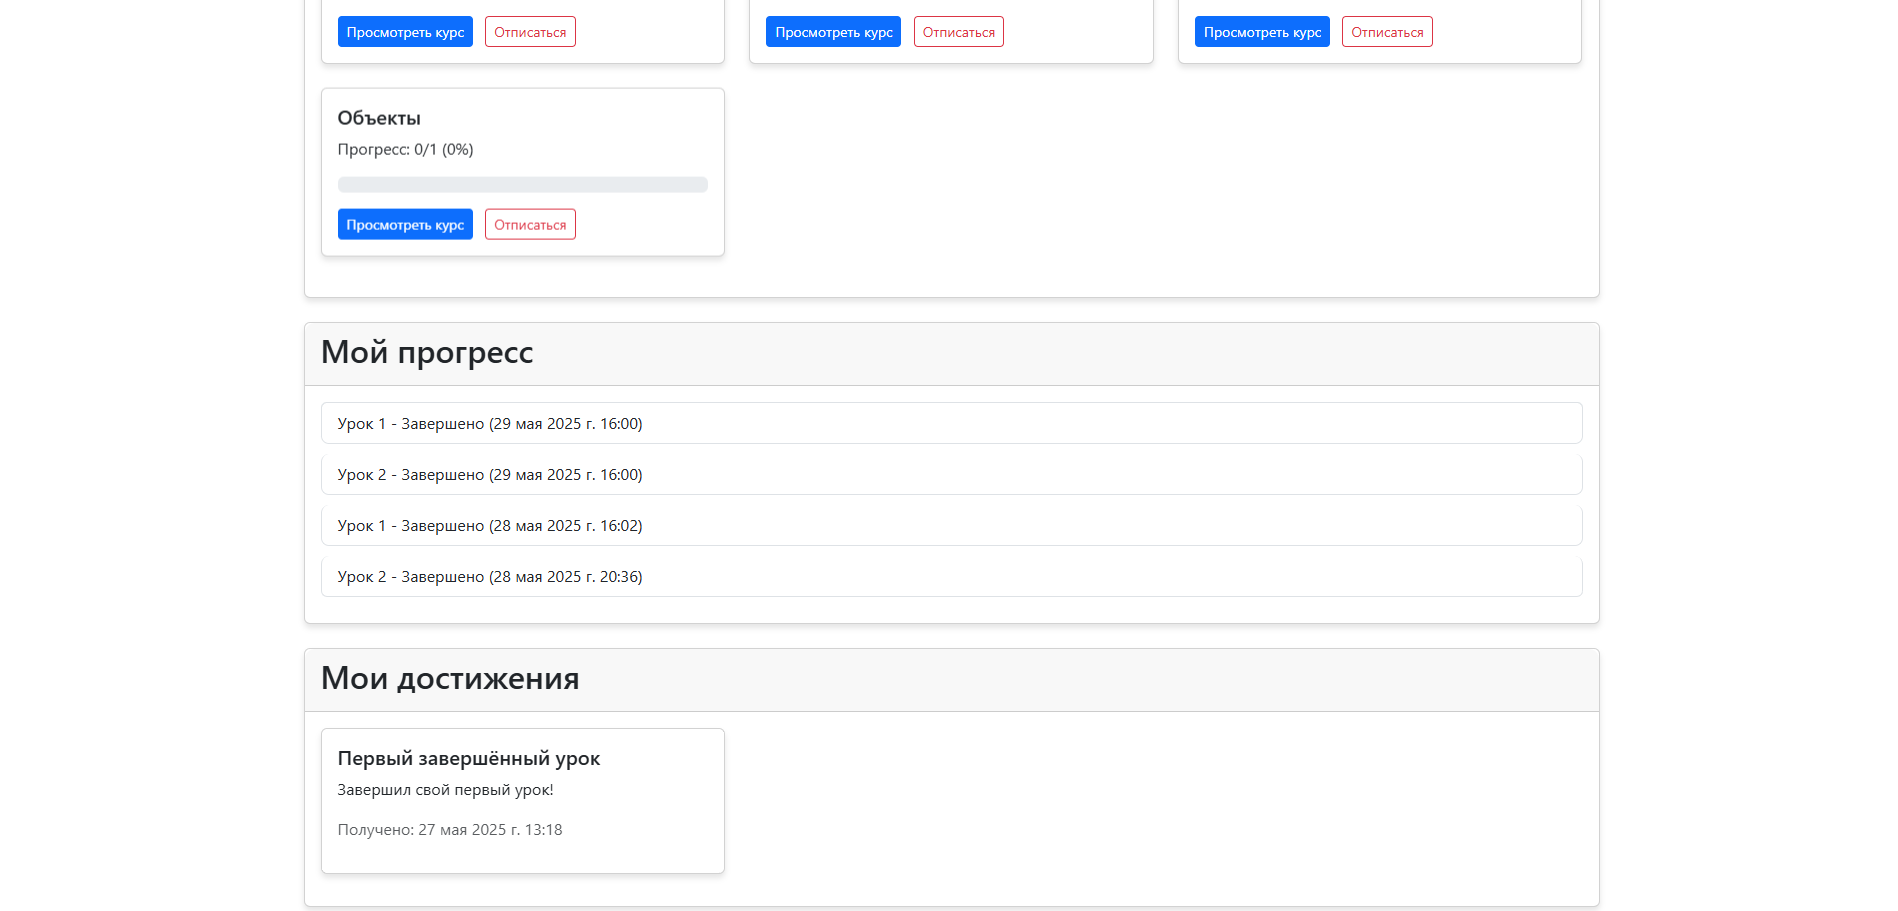
\includegraphics[width=0.9\textwidth]{images/прогресс} 
		\caption{Просмотр прогресса студента}
		\label{progress:image}
	\end{figure}
	

\subsubsection{Управление вопросами и ответами теста}
	
Описание: преподаватель должен иметь возможность добавить, редактировать и удалить вопросы и ответы теста, связанного с уроком.
	
Ожидаемый результат: вопросы и ответы успешно добавляются, редактируются или удаляются, изменения отражаются в тесте для студентов. При ошибке (например, некорректный тип вопроса) система выдает сообщение.
	
	\begin{figure}[ht]
		\centering
		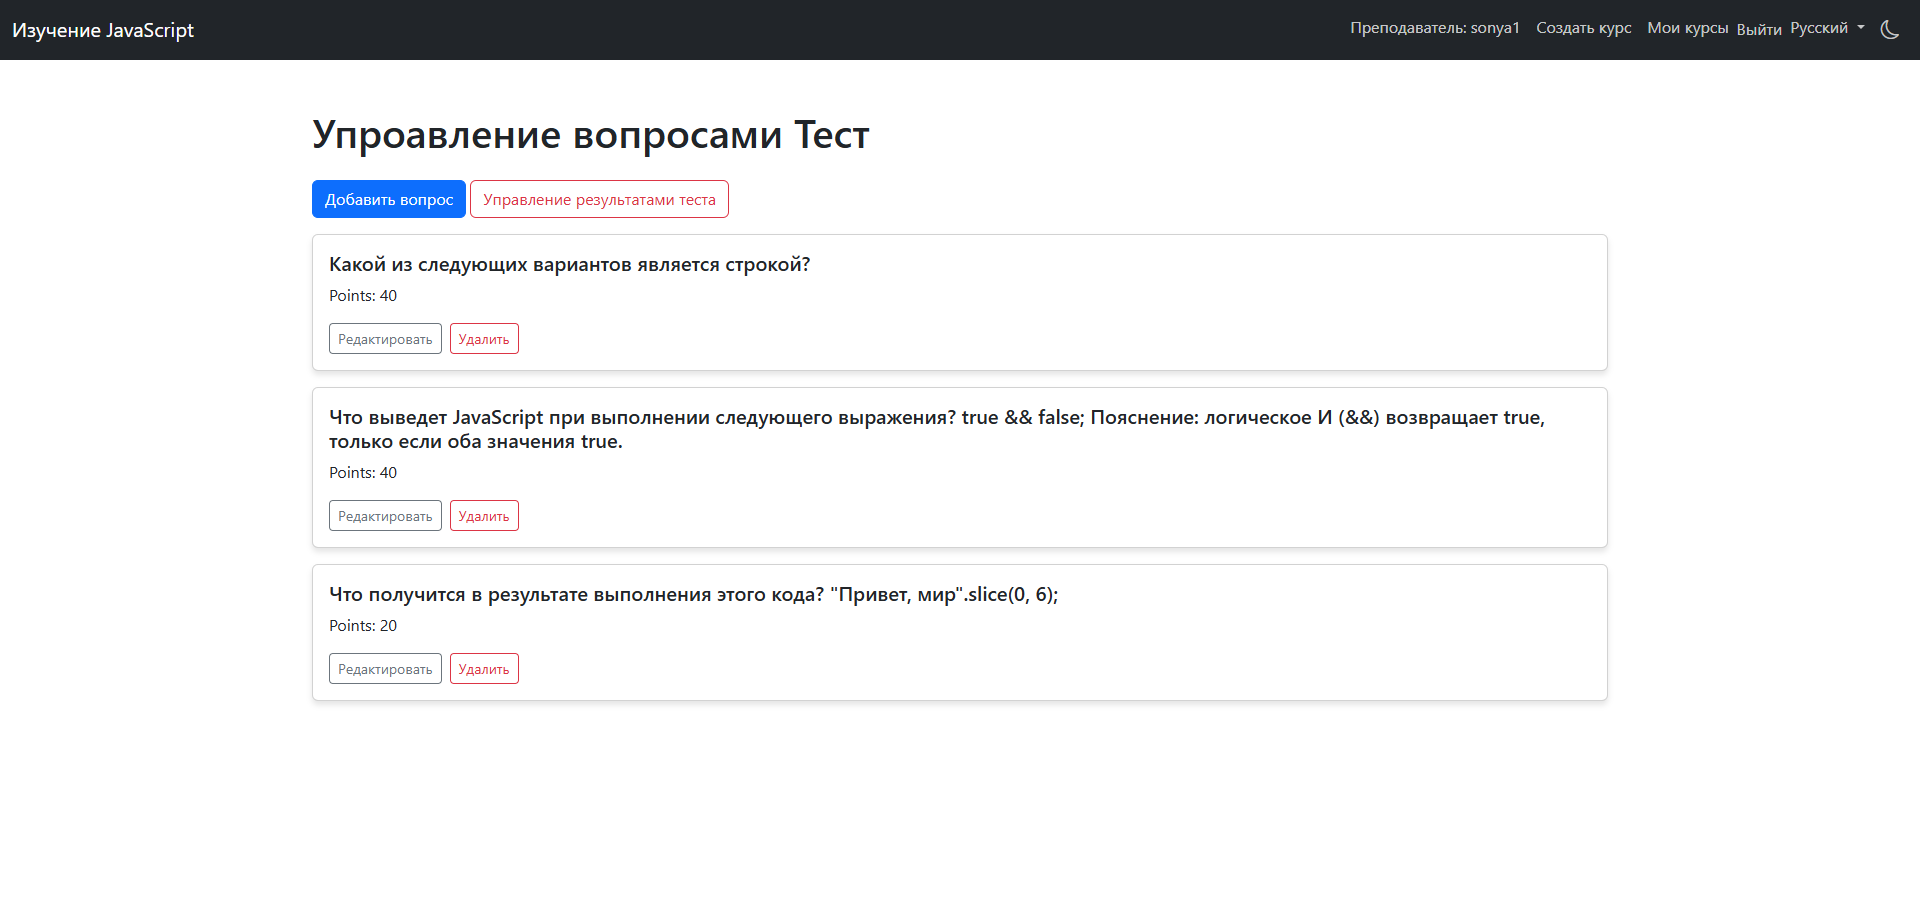
\includegraphics[width=0.9\textwidth]{images/вопросы} 
		\caption{Управление вопросами и ответами теста}
		\label{questions:image}
	\end{figure}

\begin{xltabular}{\textwidth}{|X|l|X|}
	\caption{Результаты системного тестирования\label{tab:system_testing_results}}\\
	\hline
	Сценарий & Статус & Описание \\ \hline
	\endfirsthead
	\continuecaption{Продолжение таблицы \ref{tab:system_testing_results}}\\
	\hline
	Сценарий & Статус & Описание \\ \hline
	\endhead
	Регистрация и авторизация & Успешно & Пользователи регистрируются и входят \\ \hline
	Создание и запись на курс & Успешно & Курс создаётся, студенты записываются \\ \hline
	Добавление урока & Успешно & Урок добавляется, контент отображается \\ \hline
	Прохождение теста & Успешно & Тесты проходятся, результаты сохраняются \\ \hline
	Присвоение достижения & Успешно & Достижение присваивается, отображается в профиле \\ \hline
	Редактирование курса & Успешно & Курс редактируется, изменения сохраняются \\ \hline
	Удаление курса & Успешно & Курс и связанные данные удаляются \\ \hline
	Переупорядочивание уроков & Успешно & Уроки переупорядочиваются корректно \\ \hline
	Проверка доступа к уроку & Успешно & Доступ ограничивается по условиям \\ \hline
	Просмотр прогресса студента & Успешно & Прогресс отображается в панели студента \\ \hline
	Управление вопросами и ответами & Успешно & Вопросы и ответы редактируются корректно \\ \hline
\end{xltabular}

Результаты: все сценарии выполнены успешно, система работает стабильно, критических ошибок не выявлено. Функциональность соответствует заявленным требованиям, обеспечивая удобство использования для преподавателей и студентов в рамках образовательных процессов. Тестирование подтвердило надежность платформы, включая обработку ошибок, ограничение доступа и управление контентом курсов.

\subsection{Сборка компонентов системы}

Для сборки и запуска веб-приложения нужно выполнить следующие шаги:

\begin{enumerate}
	\item Установка окружения:
	\begin{itemize}
		\item установите Python 3.9+ и pip.
		\item склонируйте репозиторий: git clone https://github.com/Seduk23/DiplomFinal.git;
		\item перейдите в директорию проекта: cd DiplomFinal;
		\item создайте и активируйте виртуальное окружение: python -m venv venv и venv\textbackslash Scripts\textbackslash activate (Windows) или source venv/bin/activate (Linux/macOS);
		\item установите зависимости: pip install -r requirements.txt.
	\end{itemize}
	
	\item Настройка базы данных:
	\begin{itemize}
		\item используется SQLite по умолчанию. Для PostgreSQL настройте settings.py и установите psycopg2-binary;
		\item выполните миграции: python manage.py makemigrations и python manage.py migrate.
	\end{itemize}
	
	\item Настройка окружения:
	\begin{itemize}
		\item создайте файл .env с настройками: SECRETKEY=yoursecretkey, DEBUG=True.
	\end{itemize}
	
	\item Подключение библиотек:
	\begin{itemize}
		\item CKEditor: установлен через pip install django-ckeditor;
		\item AOS и Bootstrap: подключены через CDN в base.html.
	\end{itemize}
	
	\item Настройка медиафайлов:
	\begin{itemize}
		\item в settings.py добавьте: MEDIAURL='/media/', MEDIAROOT=BASEDIR / 'media'.
	\end{itemize}
	
	\item Локализация:
	\begin{itemize}
		\item настройте LANGUAGES и LOCALEPATHS в settings.py;
		\item скомпилируйте переводы: python manage.py compilemessages.
	\end{itemize}
	
	\item Запуск:
	\begin{itemize}
		\item соберите статические файлы: python manage.py collectstatic;
		\item создайте суперпользователя: python manage.py createsuperuser;
		\item запустите сервер: python manage.py runserver.
	\end{itemize}
\end{enumerate}